\documentclass[11p,oneside]{book}
\usepackage{amsmath}
\usepackage{amssymb}
\usepackage{fontspec}
\usepackage{geometry}
\usepackage{pdfpages}
\usepackage{subfigure}
\usepackage{geometry}
\usepackage{graphicx}
\usepackage{emptypage}
\usepackage{float}
\usepackage[dvipsnames]{xcolor}

\title{\Huge\textbf{The Thinking Machine Chronicle} \\[1.5cm]
       \Large\textit{Exploring the Evolution of Artificial Intelligence}}
\author{\Large\textbf{郁孜欣} \\[3cm]
\date{Shanghai, 2024}
}

\setmainfont{Palatino}
\geometry{a4paper,scale=0.7}
\linespread{1.2}

\begin{document}

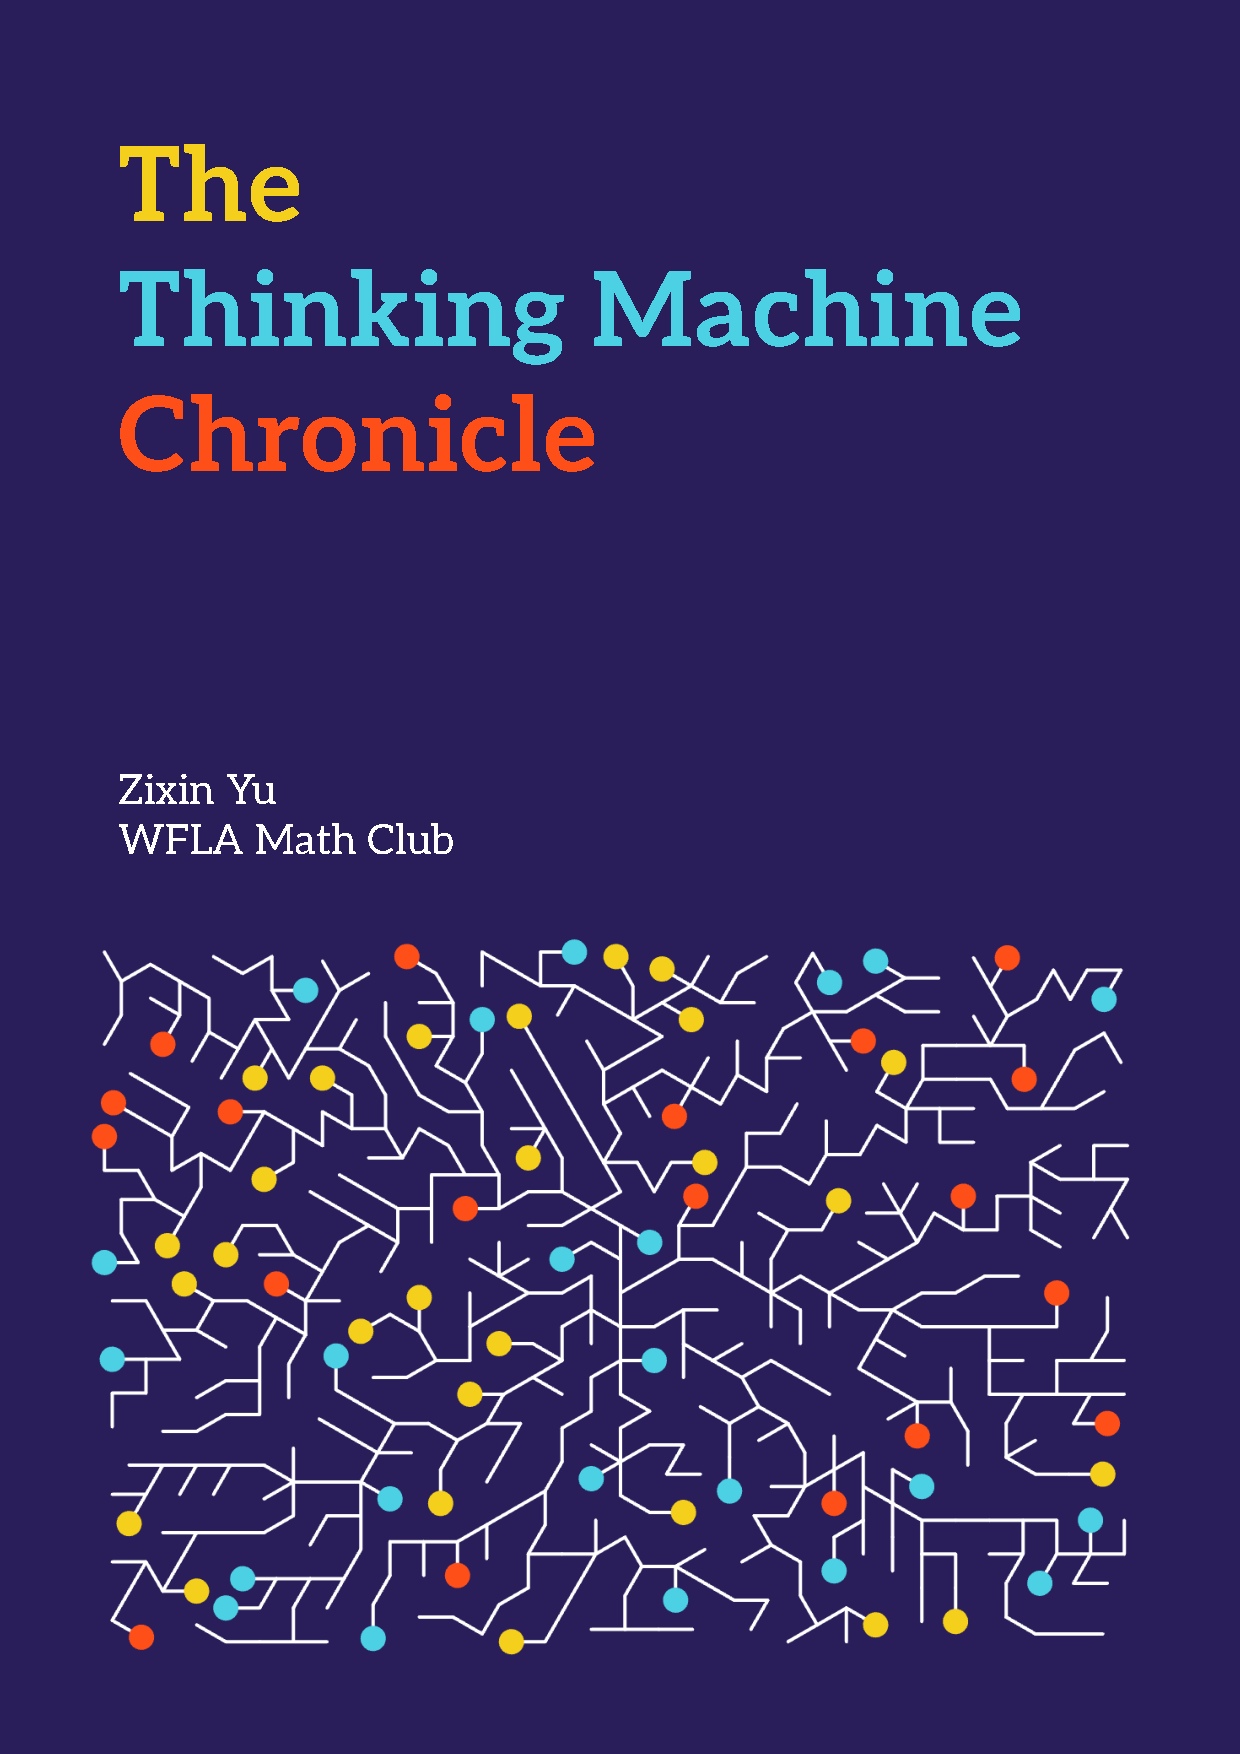
\includepdf{tmc_cover.pdf}
\maketitle

\begingroup
\let\cleardoublepage\clearpage
\tableofcontents
\endgroup
\thispagestyle{empty}

\makeatletter\@openrightfalse

\part{Basic Models}

\chapter{The Earliest Neural Network: MP Model}

\section{Introduction}

If we were currently in a general introduction to artificial intelligence class, I believe the teacher would likely start with artificial neural networks (ANNs) and use the structure on the right of the figure to explain what input layers, hidden layers, and output layers are. The weighted sum of the neuron’s output, passed through an activation function $f$, seems to align well with our intuitive understanding of biomimetic structures and the general mechanism of neurons generating pulses. However, how did scientists abstract the complex circuits of neural activity (as shown on the left of the figure) into the concise form of ANNs? 
\\

The answer to this question lies in the widely recognized early work published in 1943, “A Logical Calculus of the Ideas Immanent in Nervous Activity.” The main contribution of this paper is the proposal of an idealized neuron model based on logical operations, enabling neurons to process information through threshold responses. It also demonstrated that neural networks could simulate any mechanical computation process and its invariance from a macroscopic perspective. In short, as depicted in Figure 1.1, the complexity of neurophysiological processes is greatly simplified into the form of logical propositions.

\begin{figure}[H]
        \centering
        \includegraphics[scale=0.4]{images/tbto_11.png}
\end{figure}

\subsection*{Preliminaries: Predicates, Functors, and Logical Connectives}

\subsubsection*{Predicates}

\textbf{Predicates} are tools in logic for describing the attributes and relations of objects. A unary predicate describes the property of a single object, containing only one variable, typically represented in the form $P(x)$. For example, let $P(x)$ represent "x is red," so if $x$ is an apple, $P(x)$ indicates that this apple is red. 
\\

Binary and multiary predicates describe relationships between objects. For instance, $R(x, y)$ can represent $x > y$, so $R(5, 3)$ indicates that 5 is greater than 3. Similarly, $Pr(N_1, N_2, \ldots, N_p, z)$ might denote the activity state of neurons $c_1, c_2, \ldots, c_p$ at time $z$.

\subsubsection*{Functors}

\textbf{Functors} are tools for establishing connections between different categories. In category theory, a category consists of objects and morphisms; objects can be anything, while morphisms are mappings that preserve structure between objects. Imagine two different cities, each with its own set of streets and buildings. The streets and buildings in each city can be seen as a “category.” In each category, streets (corresponding to morphisms) connect buildings (corresponding to objects). The layout of streets and buildings may differ completely between cities.
\\

A functor acts as a highly detailed map, not only showing the corresponding location of each building in another city but also explaining the corresponding route (street) in the other city. In other words, a functor is a rule that maps objects and morphisms in one category to objects and morphisms in another category while preserving relationships (maintaining the structure of the category). In comparison, a function only acts on objects, describing a simple mapping relationship between two sets.
\\

Suppose there are two categories representing position and temperature. For example, $te(3) = 5$ indicates that the temperature at position 3 is 5. Here, positions and temperatures form a category, where objects are positions, and morphisms are mappings from positions to temperature values.
\\

These two concepts may sound complex, but they are not difficult. Predicates describe relationships or states between objects, while functors are mappings between categories. When we input a property value, we get the value of a new property in return.
\\

We often use propositional variables $P, Q, R$ to represent basic propositions or statements. Here are the five fundamental logical connectives:

\begin{itemize}
    \item $\lnot$ Negation, representing “not”; $\lnot P$ means “not $P$.”
    \item $\land$ Conjunction, representing “and”; $P \land Q$ means “both $P$ and $Q$ hold.”
    \item $\lor$ Disjunction, representing “or”; $P \lor Q$ means “at least one of $P$ or $Q$ holds.”
    \item $\rightarrow$ Implication, representing “if…then…”; $P \rightarrow Q$ means “if $P$ holds, then $Q$ also holds.”
    \item $\leftrightarrow$ Biconditional, representing “if and only if”; $P \leftrightarrow Q$ means “$P$ holds if and only if $Q$ holds.”
\end{itemize}

In Carnap’s book, $\lnot$ is written as $~$, and $\land$ as $\cdot$ (note that in the next article, we’ll switch to the commonly used symbols). $\sum$ denotes the disjunction of multiple logical propositions, while $\prod$ denotes the conjunction of multiple logical propositions. $\equiv$ indicates the equivalence of two logical expressions.
\\

Now we can proceed to analyze the paper. The article begins with several key points in the Introduction:

\begin{enumerate}
    \item Neural activity has an "all-or-none" nature (neural activity is either present or absent, akin to 0 or 1, true or false).
    \item To trigger a pulse in the next neuron, a certain number of synapses must activate within a specific time frame (each neuron has a threshold independent of its position and previous activity).
    \item The only significant delay in the nervous system is synaptic conduction delay (axon delay can be ignored).
    \item Inhibitory synapses prevent neuron activation at certain times (explains the refractory period of neurons using inhibitory synapses).
    \item The structure of neural networks does not change over time (long-term phenomena like learning and extinction are broadly equivalent to the original network).
\end{enumerate}

\section*{Definitions}

We first define a functor $S$ whose value for a given property $P$ is the property held when $P$ satisfies its predecessor. The expression is given by
\[
S(P)(t) = P(Kx), \quad t = x'
\]
where $K$ is a numerical operator, and $t$ denotes the successor of $x$. This expression may look complex, but it essentially means that $S(P)(t) = P(t-1)$. Here, the parameter in the parentheses on the left side is often omitted, making it a predicate, $[\mathbf{Pr}]$, and $S^2 \mathbf{Pr} = S(S(\mathbf{Pr}))$.
\\

Now, we define the structure of a neural network $\mathcal{N}$, which includes neurons $c_1, c_2, \ldots, c_n$. Let $N_i(t)$ represent the state of neuron $c_i$ at time $t$, describing whether neuron $c_i$ fires at time $t$. Sometimes, we use the object language and denote it as $N_i$. The boundary neurons of $\mathcal{N}$ are defined as neurons without axons connecting to their synapses. **Boundary neurons do not receive synaptic connections, so their input signals act directly on other parts of the network, unaffected by other neurons in the network ("inputs"). This property allows us to break down complex neural activities into simpler components for understanding**. Let $N_1, \ldots, N_p$ represent the boundary neurons and $N_{p+1}, \ldots, N_n$ represent the other neurons. The solution of such a neural network takes the form:
\[
S_i: N_{p+1}(z_1) \equiv Pr_i(N_1, \ldots, N_p, z_1)
\]
where $Pr_i$ contains only one free variable $z_1$ and may include some constant sentences $[\mathbf{sa}]$. Furthermore, each $S_i$ holds for $\mathcal{N}$. Next, we define two key terms: narrow realizability and extended realizability.

\begin{figure}[H]
    \centering
    \includegraphics[scale=0.7]{images/tbto_12.png}
\end{figure}

Oppositely, consider a predicate $Pr_1(^1{p_1}^1, ^1{p_2}^1, \ldots, ^1{p_p}^1, z_1, s)$. It is called narrowly realizable if there exists a network $\mathcal{N}$ with a series of $N_i$ such that $N_1(z_1) \equiv Pr_1(N_1, N_2, \ldots, z_1, sa_1)$ holds. Subsequently, we define extended realizability, meaning that $S^n(Pr_1)(p_1, \ldots, p_p, z_1, s)$ is narrowly realizable for some $n$.
\\

To interpret these definitions, narrow realizability is a stringent condition requiring a specific neural network structure to directly achieve a particular state described by the predicate through specific neuron arrangements and input substitutions. Conversely, extended realizability is a more lenient condition, allowing multiple applications of functor $S$ to transform and expand propositions until the expanded proposition is narrowly realizable.

\begin{figure}[H]
    \centering
    \includegraphics[scale=0.4]{images/tbto_13.png}
\end{figure}

Let’s consider a simple example as shown above. First, take the expression $N_3(z_1) \equiv Pr_(N_1, N_2, z_1)$. Since $N_3(t) \equiv N_1(t-1) \land N_2(t-1)$, this neural network is narrowly realizable by the i.n.s. definition. For $N_5(z_1) \equiv Pr(N_1, N_2, z)$, this expression is not directly realizable. Still, we can utilize intermediate neurons cleverly to derive a neural network since $N_5(t) \equiv N_4(t-1) \lor N_3(t-1)$, and according to $N_3(t) \equiv N_1(t-1) \land N_2(t-1)$, we get $N_5(t) \equiv N_1(t-2) \land N_2(t-2)$. As $S^2 Pr$ is narrowly realizable, $Pr$ is extendedly realizable.
\\

Finally, we arrive at the last definition! The paper defines Temporal Propositional Expressions (TPE) using recursive rules.

\begin{figure}[H]
    \centering
    \includegraphics[scale=0.4]{images/tbto_14.png}
\end{figure}

First, $p[z_1]$ is the basic temporal propositional expression, where $p_1$ is a predicate variable and $z_1$ is a time point. Secondly, the definition states that the result of applying functor $S$, logical “or,” “and,” or “not” operations to TPEs $S_1$ and $S_2$ is still a TPE. Lastly, apart from the above forms, no other forms constitute TPEs—this ensures the completeness of the definition.

\section*{Review}

We defined functor $S$, solutions for neural networks, narrow and extended realizability, and TPEs. Before moving on to proofs and examples, let’s review the core questions:
\begin{enumerate}
    \item Find an effective method to obtain a computable set of $S$ that forms the solution for any given network (calculate the behavior of any network).
    \item Describe a set of realizable solutions.
\end{enumerate}

In simple terms, the problems are (1) to calculate any network's behavior and (2) to determine networks that manifest as specific states.

\section*{Theorems and Simple Proofs}

\textbf{Note 1:} A 0th-order neural network refers to a network without circular structures. The latter half of the paper provides detailed explanations for nets with circles, which are not covered here.

\subsection*{Theorem 1}
\textit{Every 0th-order net can be solved in terms of Temporal Propositional Expressions (TPEs).}
\\

Let $c_i$ be any neuron in $\mathcal{N}$ with a threshold $\beta_i > 0$. Let $c_{i1}, c_{i2}, \ldots, c_{ip}$ represent the neurons with excitatory synapses on $c_i$, with synaptic weights $n_{i1}, n_{i2}, \ldots, n_{ip}$. Let $c_{j1}, c_{j2}, \ldots, c_{jq}$ represent the neurons with inhibitory synapses on $c_i$. Let $\kappa_i$ be the class of subsets of $\{n_{i1}, n_{i2}, \ldots, n_{ip}\}$ such that the sum of these subsets exceeds $\beta_i$ (capable of activating $c_i$). Based on the assumptions introduced in the Introduction, we can write
\[
N_i(z_1) \equiv S \left\{\prod_{m=1}^q \lnot N_{jm}(z_1) \land \sum_{\alpha \in \kappa_i} \prod_{s \in \alpha} N_{is}(z_1) \right\}
\]
where $\sum$ and $\prod$ represent finite disjunction and conjunction, respectively. This expression may look complex, but its meaning is simple. It states that neuron $c_i$ fires at time $z_1$ if and only if at time $z_1 - 1$, none of the inhibitory neurons are firing and there exists a subset of excitatory neurons whose cumulative pulse value exceeds the threshold $\beta_i$, as illustrated in the figure below.

\begin{figure}[H]
    \centering
    \includegraphics[scale=0.45]{images/tbto_15.png}
\end{figure}

Assuming a threshold of two, it’s clear that $N_4$ firing requires both $N_1$ and $N_2$ to be true (i.e., $c_1$ and $c_2$ fired in the previous moment) and $N_3$ to be false (i.e., the inhibitory neuron $c_3$ was not activated). Since such an expression can be written for each non-boundary neuron, we can replace each $N_{jm}$ and $N_{is}$ with their equivalent expressions until $N_i(z_1)$ is entirely equivalent to a propositional logic expression formed by boundary neurons, thus deriving the solution of a neural network.

\subsection*{Theorem 2}
\textit{Every TPE is realizable by a 0th-order network in the extended sense.}
\\

\noindent \textbf{Note 2:} The term “realizable in the extended sense” is abbreviated as “realizable” in the proof.
\\

The second theorem states that for any neuron state description, there exists a 0th-order network that realizes it in the extended sense. The proof of Theorem 2 provides a recursive method for constructing a 0th-order network that realizes a TPE.
\\

Since functor $S$ essentially acts as a time operator, it commutes with basic logic operations (disjunction, conjunction, negation). Thus, if network $\mathcal{N}$ can realize $S_i$ at the current time, we can achieve $S_i$ at the previous time by introducing appropriate delay neurons. Let’s look at an example:
\\

Consider a proposition $S_i = p_1(z_1) \lor p_2(z_1)$, and suppose $S_i$ is narrowly realizable. Applying the functor $S$ and using its commutativity with logic operations, we get
\[
S(S_i) = S(p_1(z_1) \lor p_2(z_1)) = S(p_1(z_1)) \lor S(p_2(z_1))
\]
$S$ is a time operator, so $S(p_1(z_1))$ and $S(p_2(z_1))$ describe the states of $p_1(z_1)$ and $p_2(z_1)$ at the previous time point. By extending network $\mathcal{N}$ with appropriate delay neurons, we can realize $SS_i$ in the narrow sense.

\begin{figure}[H]
    \centering
    \includegraphics[scale=0.6]{images/tbto_16.png}
\end{figure}

Thus, if $S_i$ is narrowly realizable, its result after $n$ applications of $S$ is still narrowly realizable because we can add intermediate neurons indefinitely. If $S_1$ and $S_2$ are both narrowly realizable, then $S^m S_1$ and $S^n S_2$ are also narrowly realizable. Now consider the four basic components of neural networks: $S(p_1(z_1))$, $S(p_1(z_1) \lor p_2(z_1))$, $S(p_1(z_1) \land p_2(z_1))$, and $S(p_1(z_1) \land \lnot p_2(z_1))$ (Figure 7), all of which are narrowly realizable.\\


\begin{figure}[H]
    \centering
    \includegraphics[scale=0.7]{images/tbto_17.png}
\end{figure}

Based on the previous conclusions, $S^{m+n+1}(p_1(z_1))$, $S^{m+n+1}(p_1(z_1) \lor p_2(z_1))$, $S^{m+n+1}(p_1(z_1) \land p_2(z_1))$, and $S^{m+n+1}(p_1(z_1) \land \lnot p_2(z_1))$ are also narrowly realizable. By the definition of extended realizability, these primitive propositions are extendedly realizable. By logically combining these basic structures, more complex neural networks can be realized in the extended sense, enabling the realization of any TPE.

\subsection*{Theorem 3}
\textit{Let there be a complex sentence $S_1$ built up in any manner out of elementary sentences of the form $p(z_1-zz)$, where $zz$ is any numeral, by any of the propositional connections: negation, disjunction, conjunction, implication, and equivalence. Then $S_1$ is a TPE if and only if it is false when its constituent $p(z_1-zz)$ are all assumed false—i.e., replaced by false sentences—or that the last line in its truth table contains an 'F', or there is no term in its Hilbert disjunctive normal form composed exclusively of negated terms.}
\\

Though complex at first glance, Theorem 3 provides the criterion for determining whether an expression is a TPE. In other words, it gives a method for determining if an expression is a TPE. There are three equivalent methods:
\begin{enumerate}
    \item The composite sentence is false when all its basic sentences are false.
    \item The last line of the truth table contains “false.”
    \item There is no term in its Hilbert Disjunctive Normal Form (HDNF) composed solely of negated terms.\\
\end{enumerate}

Let’s examine a few examples for each condition:
\begin{enumerate}
    \item For the composite sentence $S_1 = p(z_1 - 1) \land q(z_1 - 2)$, where $p(z_1 - 1)$ and $q(z_1 - 2)$ are basic propositions. When both $p(z_1 - 1)$ and $q(z_1 - 2)$ are false, $S_1$ is also false, i.e., $S_1 = \text{False} \land \text{False} = \text{False}$. Therefore, $S_1$ satisfies the first condition and is a TPE.
    \item For the composite sentence $S_2 = p(z_1 - 1) \lor q(z_1 - 2)$, the truth table is as follows:
    
\begin{figure}[H]
        \centering
        \includegraphics[scale=0.4]{images/tbto_18.png}
 \end{figure}
    
    As shown, when both $p(z_1 - 1)$ and $q(z_1 - 2)$ are false, $S_2$ is also false. Hence, $S_2$ satisfies the second condition.
    \item For the composite sentence $S_3 = \neg p(z_1 - 1) \land \neg q(z_1 - 2)$, converting it to HDNF gives $S_3 = \neg p(z_1 - 1) \land \neg q(z_1 - 2)$. In HDNF, the only term $\neg p(z_1 - 1) \land \neg q(z_1 - 2)$ consists solely of negated terms. Therefore, $S_3$ does not meet the third condition and is not a TPE.
\end{enumerate}

\section*{Application to Neural Networks}

Let’s apply these theorems to implement a neural network. Consider a scenario: when an ice cube touches and then leaves our skin for a moment, we feel heat before coolness; but if it stays longer, we only feel a chill. To model this situation, let $N_1$ and $N_2$ represent “heat” and “cold” receptors, respectively, and let $N_3$ and $N_4$ represent neurons sensing heat and cold. We assume that $N_4$ senses cold only if the cold touch persists for two time units, yielding the following sentences:

\begin{align*}
&N_3(t) \equiv N_1(t-1) \lor N_2(t-3) \land \lnot N_2(t-2) \\
&N_4(t) \equiv N_2(t-2) \land N_2(t-1)
\end{align*}

Since these sentences are already in Hilbert Disjunctive Normal Form (HDNF), Theorem 3 indicates that both $N_3(t)$ and $N_4(t)$ are TPEs. Given this, Theorem 2 can construct a neural network in the following form:

\begin{figure}[H]
    \centering
    \includegraphics[scale=0.6]{images/tbto_19.png}
\end{figure}

Finally, the paper mentions that different inhibition phenomena are broadly equivalent (2) extinction and learning are equivalent to absolute inhibition. If these two conclusions are proven, it indicates that the current structure simulates actual neural networks, allowing us to compute any network’s behavior and determine networks manifesting specific states. This part is briefly discussed in the original paper, so we will not explain the details here.

\section*{Summary}

The McCulloch-Pitts neuron model simplifies neuron behavior into logical operations, executing basic logic through "all-or-none" responses. Its significance lies in formalizing the behavior of neural systems, demonstrating the Turing completeness of neural networks, capable of simulating any state. This groundbreaking theory laid a solid foundation for the Perceptron and propelled the development of artificial neural networks (ANNs). 

\section*{References}

\begin{enumerate}
    \item McCulloch, W. S., \& Pitts, W. (1943). A logical calculus of the ideas immanent in nervous activity. \textit{The Bulletin of Mathematical Biophysics}, \textit{5}(4), 115–133. https://doi.org/10.1007/bf0
    2478259
    \item Marshall, M. (2021, June 7). \textit{Google has mapped a piece of the human brain in the most detail ever.} New Scientist. https://www.newscientist.com/article/2279937-google-has-mapped-a-piece-of-human-brain-in-the-most-detail-ever/
    \item \textit{A Friendly Introduction to [Deep] Neural Networks | KNIME}. (2021). KNIME. 
\end{enumerate}

\chapter{The First Intelligent Machine: Perceptron}

\section*{Preface}

Continuing from the last article, we’ll delve into a pioneering work in the field of artificial intelligence that followed the MP neuron model: the \textbf{Perceptron}. This article will give a detailed analysis of the 1957 paper, \textit{The Perceptron: A Probabilistic Model for Information Storage and Organization in the Brain}, by Frank Rosenblatt, a psychologist and neuroscientist at Cornell University.

\section*{Introduction}

At the beginning of the article, the author presents three fundamental questions for understanding cognition, generalization, memory, and thought: 
\begin{enumerate}
    \item How do biological systems perceive or detect information from the physical world?
    \item In what form is information stored in memory?
    \item How does stored information influence recognition and behavior?
\end{enumerate}

The first question has largely been addressed in sensory physiology. For the second and third questions, the author discusses two perspectives: \\

\textbf{The Coded Memory Hypothesis} suggests that information is stored in an encoded form, like a wiring diagram, that can directly translate sensory input into memory. Recognizing external stimuli involves matching the current sensory pattern with stored content and mapping it to a corresponding response. \\

\textbf{The Empiricist Memory Hypothesis} proposes that information storage does not involve specific encoding but occurs through forming new connections in the nervous system. Since the information is stored as neural connections, new stimuli use these established pathways, triggering an appropriate response without needing a separate recognition process. \\

\begin{figure}[H]
    \centering
    \includegraphics[scale=0.2]{images/tbto_21.png}
\end{figure}

These two hypotheses can actually be mapped to two major schools of artificial intelligence: \textbf{Connectionism} and \textbf{Symbolism}. Symbolism assumes cognitive processes are achieved through clear symbol manipulation and sequential application of rules. In contrast, Connectionism models cognition by simulating neural networks, relying on distributed representations and statistical methods. \\

In the previous article, we discussed MP neurons, which are based on Boolean logic and binary operations. In the \textit{Perceptron} paper, the author critiques symbolic methods. These theorists focus on implementing functions like perception and memory using deterministic physical systems rather than studying how the brain actually performs them. Many of the proposed models fail in important ways: they lack consistency across different situations (equivalence), they don’t use neural resources efficiently (neuroeconomy), they impose strict requirements on connections (excessive specificity), and the variables in the models lack biological evidence. Supporters of these physical systems argue that biological intelligence can be replicated by improving existing principles. \textbf{However, the author believes these limitations show that models not based on biological systems can never explain biological intelligence, as the difference in principles is clear.} \\

Conversely, studies that focus on biological systems often lack precision and rigor, making it difficult to assess whether the described systems can actually work in real neural networks. \textbf{The lack of an analytical language as effective as Boolean algebra is another obstacle.} \\

To address these issues, the author first introduces several key assumptions:
\begin{enumerate}
    \item The construction of the neural system’s initial network is largely random, with minimal genetic restrictions.
    \item Neural connections exhibit some plasticity. After a period of neural activity, the probability of stimulating one group of cells and triggering a response in another group changes due to long-term changes in neurons.
    \item Similar stimuli tend to form pathways to the same responsive cells, and vice versa.
    \item Positive and negative reinforcement promotes or inhibits the formation of connections.
    \item Similarity isn’t an inherent attribute of specific stimuli but depends on the physical organization of the perceptual system.
\end{enumerate}

These assumptions will serve as essential foundations for the model. Unlike previous work, \textbf{the Perceptron uses a probabilistic model rather than Boolean operations.}

\section*{The Basic Structure of the Perceptron}

The following is a simple diagram of the perceptron’s structure:

\begin{figure}[H]
    \centering
    \includegraphics[scale=0.4]{images/tbto_22.png}
\end{figure}

\textbf{The figure above} shows a simple diagram of the perceptron structure. The model is organized into four parts:

\begin{enumerate}
    \item \textbf{Sensory Input Layer}: The perceptron’s input comes from sensory receptors, like retinal points, labeled S-points, that respond in an "all-or-none" manner to stimuli. Note: "All-or-none" means that if the stimulus weight exceeds the neuron’s threshold $\theta$, the neuron activates; if not, it remains inactive.
    \item \textbf{Projection Area}: The S-points send signals to a projection area (a group of associated cells labeled $A_1$, with neurons referred to as A units). The activation of A units follows the same "all-or-none" rule. Notice the \textbf{localized connections} here: A units’ source points tend to cluster around each A unit’s central retinal point. The number of origin points decreases exponentially with distance from the central point. This distribution is vital in \textbf{contour detection}, making it a \textbf{bio-inspired design}. Sometimes, the projection area is omitted during modeling.
    \item \textbf{Association Area}: Each A unit in the association area receives signals from multiple source points, and connections between the two regions are \textbf{random}.
    \item \textbf{Response Layer}: Outputs from the association area go to response cells (labeled R units). While the perceptron uses feedforward connections until the association area, feedback is provided in the response layer. The author suggests two almost equivalent feedback mechanisms:
    \begin{itemize}
        \item (a) Excitatory feedback to the source cell set of an R unit.
        \item (b) Inhibitory feedback to the complement of the source set of an R unit.
    \end{itemize}
\end{enumerate}

In this system, based on feedback, the neurons’ responses are \textbf{mutually exclusive}. If one response unit $R_1$ is activated, it inhibits the set of cells connected to another response unit $R_2$, preventing $R_2$ from responding. As reinforcement and inhibition continue, the system gradually adapts to stimuli of different categories—a process we describe as \textbf{learning ability}. \\

For simplification in later analysis, only \textbf{Sensory Input - Association Area - Response Layer} are kept. The A unit represents neurons in the association area, and the R unit represents neurons in the response layer. To simplify further, the author distinguishes between two response phases:

\begin{figure}[H]
    \centering
    \includegraphics[scale=0.4]{images/tbto_23.png}
\end{figure}

The figure above depicts the response phases to stimuli.
\textbf{Response Phases:}
\begin{itemize}
    \item \textbf{Predominant Phase}: A units in the system respond to stimuli, but R units remain inactive. This phase is temporary and transitions to the Postdominant phase.
    \item \textbf{Postdominant Phase}: One R unit becomes active, dominating by suppressing other activities in its source set.
\end{itemize}

In the predominant phase, responses are random. However, as stimulus-response connections are reinforced, the system learns to respond to specific stimuli. Below, we discuss the characteristics of each neuron in the macrostructure.

\section*{Modeling Neuron Characteristics}

To address assumption two (neural plasticity) and to enable the Perceptron's dynamic learning process, we introduce a model for neuron characteristics, which will serve as the foundation for subsequent simulations. \\

Assume that each A unit’s output impulse can be represented by a value $V$, which could reflect amplitude, frequency, delay, or transmission probability. A higher value indicates that all output impulses of an A unit are more effective or more likely to reach the response layer. Each A unit’s value is assumed to be relatively stable (determined by the cell membrane and metabolic state of the cell), but it is not constant. We generally assume that \textbf{activity increases the cell’s value, while inactivity decreases it}. \\

An interesting model is one where cells compete for metabolic materials, with more active cells drawing from inactive ones. In such a system, without activity, all cells’ states would stabilize, resulting in a net value balance across the system. The author introduces three systems ($\alpha, \beta, \gamma$) with different rules for changes in neuron values $V$:

\begin{figure}[H]
    \centering
    \includegraphics[scale=0.45]{images/tbto_24.png}
\end{figure}

\textbf{The figure above} compares the logic characteristics of three systems:

\begin{itemize}
    \item \textbf{$\alpha$ System (Uncompensated Gain System)}: Each time an A unit receives a stimulus, it gets a fixed gain, accumulating over time without decreasing. This cumulative gain mechanism is suited for tasks with long-term accumulation effects.
    \item \textbf{$\beta$ System (Constant Feed System)}: Each source set gains at a constant rate, with distribution proportional to the activity in the set. Non-dominant set cells also receive gains, ensuring all units have the chance to activate and strengthen over time. This balanced mechanism supports ongoing learning and stable gain distribution.
    \item \textbf{$\gamma$ System (Parasitic Gain System)}: Active cells gain $V$ values at the expense of inactive ones, keeping the total source set value constant. This competitive mechanism is suitable for tasks focused on resource optimization.
\end{itemize}

The next section builds learning curves and performs a sensitivity analysis on the model.

\section*{Model Analysis of the Predominant Phase}

To compare learning curves, we define two key metrics:

\begin{itemize}
    \item \textbf{$P_a$}: The expected proportion of A units activated by a given stimulus. This is calculated by summing over all possible excitatory ($e$) and inhibitory ($i$) inputs under the condition that the \textbf{sum of excitation minus inhibition reaches or exceeds} the threshold $\theta$ ($e - i \geq \theta$). $P(e, i)$ represents the joint probability of excitatory and inhibitory components; $x$ is the total excitatory connections per A unit, $y$ is the total inhibitory connections, and $R$ is the proportion of S-points activated before each A unit.
    \begin{align*}
    P_a &= \sum_{e=\theta}^x \sum_{i=0}^{\min(y, e-\theta)} P(e, i) \\
    P(e, i) &= \binom{x}{e} R^e (1 - R)^{x - e} \times \binom{y}{i} R^i (1 - R)^{y - i}
\end{align*}
    \item \textbf{$P_c$}: The conditional probability that an A unit responding to a stimulus $S_1$ will also respond to a different stimulus $S_2$:
    \[
    P_c = \frac{1}{P_a} \sum_{e=\theta}^x \sum_{i=e-\theta}^y \sum_{l_e=0}^e \sum_{l_i=0}^i \sum_{g_e=0}^{x-e} \sum_{g_i=0}^{y-i} P(e, i, l_e, l_i, g_e, g_i)
    \]
    Here, $l_e$ and $l_i$ are the counts of excitatory and inhibitory source points “lost” when $S_1$ is replaced by $S_2$, while $g_e$ and $g_i$ are the counts of points “gained” when $S_1$ is replaced by $S_2$. The joint probability $P(e, i, \ell_e, \ell_i, g_e, g_i)$ is as follows:
\begin{align*}
        P(e, i, \ell_e, \ell_i, g_e, g_i) &= \binom{x}{e} R^e (1 - R)^{x - e} \times \binom{y}{i} R^i (1 - R)^{y - i} \times \binom{e}{\ell_e} L^{\ell_e} (1 - L)^{e - \ell_e} \\
        &\times \binom{i}{\ell_i} L^{\ell_i} (1 - L)^{i - \ell_i} \times \binom{x - e}{g_e} G^{g_e} (1 - G)^{x - e - g_e} \\
        & \times \binom{y - i}{g_i} G^{g_i} (1 - G)^{y - i - g_i}
\end{align*}
  
    Here, $L$ is the proportion of S-points lit by $S_1$ but not $S_2$, and $G$ is the proportion of S-points remaining from $S_1$ that are included in $S_2$. Let’s examine how $P_a$ and $P_c$ change with parameter variations.
\end{itemize}

\section*{Sensitivity Analysis of $P_a$}

Using the formula and rules discussed, we can plot graphs:

\begin{figure}[H]
    \centering
    \includegraphics[scale=0.28]{images/tbto_25.png}
\end{figure}

\textbf{The figure above} shows the variation of $P_a$ with the proportion of retina area illuminated ($R$). \\

\textbf{Conclusions:}
\begin{enumerate}
    \item Increasing the threshold $\theta$ or increasing inhibitory connections $y$ reduces $P_a$.
    \item When excitatory and inhibitory inputs are roughly balanced, the $P_a$ curve flattens with changes in $R$.
    \item Systems with similar amounts of excitatory and inhibitory input converge faster. For optimal stability, a balance of excitatory and inhibitory input is desirable.
\end{enumerate}

\section*{Sensitivity Analysis of $P_c$}

\begin{figure}[H]
    \centering
    \includegraphics[scale=0.28]{images/tbto_26.png}
\end{figure}

\textbf{The figure above} shows the variation of $P_c$ with $R$. \\

\begin{enumerate}
    \item As $\theta$ increases, $P_c$ decreases faster than $P_a$.
    \item Like $P_a$, $P_c$ decreases as the proportion of inhibitory connections $y$ increases.
\end{enumerate}

Additionally, the author explored how $P_c$ changes with stimulus overlap $C$, as shown in the following figure:

\begin{figure}[H]
    \centering
    \includegraphics[scale=0.28]{images/tbto_27.png}
\end{figure}

\textbf{The figure above} illustrates the variation of $P_c$ with $C$. Solid line represents $R=0.5$, dashed line represents $R=0.2$, with $x=10$ and $y=0$. \\

\begin{enumerate}
    \item Even when stimuli are entirely non-overlapping, $P_c$ remains above zero, showing that the system can still respond to completely different stimuli.
    \item As overlap increases, $P_c$ approaches 1, indicating strong consistency in system response.
    \item Higher threshold values result in lower $P_c$ values compared to lower thresholds.
\end{enumerate}

Analyzing $P_a$ and $P_c$ provides a theoretical basis for quantitative analysis and parameter tuning. Summing up the insights gained:

\begin{itemize}
    \item \textbf{Symbolism vs. Connectionism}: A comparison of two major schools of thought in artificial intelligence.
    \item \textbf{Transition from Formal Logic to Probabilistic Models}: The shift from Boolean logic to probabilistic operations in neural networks.
    \item \textbf{The Foundational Structure and Functioning of the Perceptron}: An explanation of the perceptron's sensory input layer, projection area, association area, and response layer.
    \item \textbf{Neuron Characteristic Modeling with Three Systems}: The $\alpha$, $\beta$, and $\gamma$ systems and their contributions to dynamic learning.
    \item \textbf{Learning Curve Development and Sensitivity Analysis}: Insights from $P_a$ and $P_c$ metrics to understand system responses.
    \item \textbf{Convergence Based on Different Criteria}: The role of excitatory and inhibitory balance in achieving neural stability and response optimization.
\end{itemize}

The second half of the original paper focuses on the perceptron’s spontaneous organization, memory and learning capabilities, and the model's performance in varied environments. We won’t cover this section here, as it primarily involves \textbf{small-scale experiments and fine-tuning} rather than the foundational contributions of the first half. \\

A major limitation of the Perceptron is that it can only solve linearly separable tasks, struggling with non-linear ones. This limitation led to the development of the \textbf{Multilayer Perceptron}, which introduced non-linear activation functions in hidden layers, allowing for non-linear classification. \\

However, challenges remain, especially with \textbf{training}. Next, we’ll explore the 1986 paper by Hinton, Rumelhart, and Williams, \textit{Learning Representations by Back-Propagating Errors}, which made training deep neural networks feasible.

\chapter{Back-propagation}

\section*{Preface}

\textbf{Preface} \\
Following the previous article in the "Tracing the Origins" series, where we explored the MP neuron, we now dive into a groundbreaking advancement in the field of AI, \textit{the Perceptron}, introduced in the 1957 paper by Frank Rosenblatt. This article will deeply analyze the 1986 paper \textit{Learning Representations by Back-Propagating Errors}~\cite{Rumelhart1986} by Rumelhart, Hinton, and others, which introduces the well-known backpropagation learning method. This method aims to minimize the discrepancy between a neural network's actual and desired outputs by adjusting connection weights within the network, thus enabling it to learn and optimize internal representations for complex tasks. This paper not only laid the theoretical foundation of modern deep learning but also sparked extensive exploration into neural networks' practical applications. At the end of this paper, the authors presented some fascinating insights from today's perspective, worth exploring further.

\section*{Introduction}

Scientists have made numerous attempts to design self-organizing neural networks. Their goal was to find an effective method for \textbf{learning and self-adjusting connections within the network} to automatically find the right connections and states for specific tasks. If inputs and outputs are directly connected, finding a way to learn is relatively straightforward: one only needs to repeatedly adjust the strength of the connections so that the output gradually approximates the target result. However, networks that directly connect outputs and inputs can only address linearly separable problems. \\

For example, if we have a basket of apples and watermelons that differ in size and dimension, we could use a straight line to separate apples and watermelons on a size-weight chart. In such problems, a line or hyperplane can fully separate data points in a 2D or multidimensional space. However, many real-world data features do not exhibit clear distinctions, such as movie review sentiment (positive or negative?) or stock market predictions (rise or fall?), which cannot be split by a simple linear boundary. \\

To tackle these linearly inseparable problems, the concept of hidden layers was proposed. The state of hidden layers is not directly given but must be learned to determine which stimuli activate neurons, layer by layer, to ensure the network produces the correct output. In the Perceptron model, although the association area sits between inputs and outputs, its connections are fixed and do not adapt through learning. In this paper, the authors found a simple yet powerful method—the backpropagation algorithm—capable of automatically adjusting hidden units to build internal representations suited to task requirements. We will first explain the core of backpropagation, introduce specific examples from the authors, and discuss algorithm improvements and intriguing questions.

\section*{Backpropagation}

This section covers the backpropagation calculation process, with the specific weight update rules explained in the next section. \\

Consider a layered network consisting of input units, an arbitrary number of hidden layers, and output units. Each layer's units set their states, beginning with the input units and working up to the output units. \textbf{The following figure} provides a simplified illustration of neuron connections and calculations in the paper:

\begin{figure}[H]
    \centering
    \includegraphics[scale=0.2]{images/tbto_31.png}
\end{figure}

The total input $x_j$ to neuron $j$ is a linear function of the outputs from connected units $y_i$ and the weights of those connections $w_{ji}$:
$$
x_j = \sum_i y_i w_{ji}
$$
where $i$ and $j$ represent the indices of neurons in the preceding and following network layers, referred to simply as "neuron $j$" and "neuron $i$." Additionally, a constant offset, known as a \textbf{bias}, may be added to the neuron’s total input. With the bias, the input can be written as:
$$
x_j = b_j + \sum_i y_i w_{ji}
$$

The real-valued output $y_j$ of the neuron is a nonlinear function of its total input $x_j$:
$$
y_j = f(x_j) = \frac{1}{1 + e^{-x_j}}
$$

The Sigmoid function is a commonly used activation function, with all output values between $(0, 1)$, and it has a straightforward derivative $\sigma'(x) = \sigma(x)(1 - \sigma(x))$. \textbf{The figure below} shows the structure of artificial neurons compared to biological neurons:

\begin{figure}[H]
    \centering
    \includegraphics[scale=0.45]{images/tbto_32.png}
\end{figure}

Our ultimate goal is to ensure that for each input vector, the network generates an \textbf{output vector that matches or closely approximates the desired output vector}. The total error $E$ of the network can be computed by comparing the actual output vector and the desired output vector:
$$
E = \frac{1}{2} \sum_c \sum_j (y_{j,c} - d_{j,c})^2
$$
where $c$ is the sample index, $j$ is the output unit index, $y$ is the actual output unit state, and $d$ is its desired state. \\

For a given data sample, the partial derivative of the error with respect to each weight is calculated through two passes. The state of each layer's units is determined by the output received from the previous layer’s units. Backpropagation, however, is more complex. Weight derivatives will propagate from the output layer down to the lower layers, using $\frac{\partial E}{\partial w}$ to adjust the weights. \textbf{The figure below} illustrates the backpropagation calculation flow:

\begin{figure}[H]
    \centering
    \includegraphics[scale=0.45]{images/tbto_33.png}
\end{figure}

\subsection*{Family Tree Network}

\begin{figure}[H]
    \centering
    \includegraphics[scale=0.45]{images/tbto_36.png}
\end{figure}

\textbf{The figure above} depicts two isomorphic family trees (left) and the activity levels in the family tree network (right). \\

Information about the family tree can be represented as triples (person1, relationship, person2), where possible relationships include father, mother, brother, sister, etc. If our network can produce the third element given the first two, it means it has successfully learned these triples. \\

The training dataset consists of binary vectors of 0s and 1s, with each person and relationship represented by a one-hot encoding. For instance, "Colin" might be represented by a one-hot vector $[1, 0, 0, \ldots, 0]$ (24 bits), while the "has-aunt" relationship might be $[0, 0, 1, \ldots, 0]$ (12 bits). The input vector is a concatenation of one-hot encoding vectors for person and relationship, forming a binary vector of length 36 (24 + 12). The family tree network training involved 1,500 passes; the first 20 passes used $\eta = 0.005$ and $\alpha = 0.5$, and the remaining used $\eta = 0.01$ and $\alpha = 0.9$. \\

The two groups of white blocks on the right side of the figure show each unit's activity level. In the first group, one active unit represents Colin; in the second group, one active unit represents the "has-aunt" relationship. Each input group is connected to a hidden layer of six units, with both hidden layers connected to a central layer of 12 units, transitioning to the penultimate layer of six units. This layer's activity will activate the correct output unit, with each output unit representing a specific person (person 2). The two black dots in the white box mean that (Colin)(has-aunt) has two correct answers—Colin has two aunts.

\subsection*{Iterative Network and Equivalent Neural Networks}

\begin{figure}[H]
    \centering
    \includegraphics[scale=0.5]{images/tbto_37.png}
\end{figure}

\textbf{The figure above} illustrates a recurrent neural network and its equivalent layered neural network. \\

In the recurrent neural network, each weight update corresponds to a layer in the equivalent layered network. When creating a layered structure equivalent to a recurrent network, two challenges arise:
\begin{enumerate}
    \item \textbf{Storing Each Unit’s Output State History}: In the layered network, intermediate layer outputs are necessary during backpropagation. Therefore, in an iterative network, each unit’s output state history needs to be stored for use in backpropagation.
    \item \textbf{Ensuring Weight Consistency}: To maintain equivalence between the layered and iterative networks, weights between different layers must have the same value. This can be achieved by averaging each corresponding weight’s $\frac{\partial E}{\partial w}$ value and adjusting each weight in proportion to the average gradient:
    $$
    \Delta w = \frac{\eta}{n} \sum_{i=1}^n \frac{\partial E}{\partial w_i}
    $$
\end{enumerate}
With these two modifications, the learning process described above can be applied directly to iterative networks.

\section*{Conclusion}

The models and cases discussed in this paper demonstrate the remarkable ability of the backpropagation algorithm to enable neural networks to learn complex, nonlinear patterns. This straightforward algorithm laid the groundwork for many modern deep learning techniques. \\

At the end of the paper, the authors note: the forward-propagation–loss-calculation–backpropagation learning process may not be entirely plausible from a biological perspective, but it performs exceptionally well in practice. Therefore, we must continue searching for algorithms that more accurately reflect biological principles. \\

From today’s perspective, advanced architectures like ResNet and Transformer, along with many optimization algorithms, bear little relation to biology or neuroscience. Yet, this raises a question: has artificial intelligence taken the wrong path? Does achieving true artificial general intelligence (AGI) require a closer connection to neuroscientific evidence? Could interdisciplinary collaboration between biology, philosophy, and computer science offer answers to these challenges in the future? \\

While these are profound questions, separating \textbf{artificial intelligence} from \textbf{intelligence} might be crucial for our research. "Artificial intelligence" often pulls us into ethical and technological debates, yet it may be misleading as a term. Intelligence encompasses reasoning, computation, decision-making, emotions, and consciousness, while neural networks can also be described as "input-hidden-output models based on error calculation and parameter optimization." \\

On one hand, responsibly applying AI is an urgent practical question. On the other, whether humanity needs to replicate intelligent, conscious entities remains debatable. Nonetheless, AI provides a valuable foundation to explore intelligence and consciousness quantitatively, even if it clears just a small patch of the clouded sky.

In the next article, we will explore the 1979 work \textit{Neocognitron}, the foundation of convolutional neural networks and computer vision. After covering these basic models, we will delve into interdisciplinary discussions on AI, neuroscience, and philosophy.

\section*{References}

\begin{enumerate}
    \item Rumelhart, D. E., Hinton, G. E., \& Williams, R. J. (1986). Learning representations by back-propagating errors. \textit{Nature}, \textit{323}, 533–536. https://doi.org/10.1038/323533a0
\end{enumerate}

\chapter{Cognitron: The Concept of Vision}

\section*{Introduction}

In the last article on the perceptron, we discussed how the backpropagation algorithm adjusts the states of hidden units, allowing neural connections to learn and adapt their states, thus solving linearly inseparable problems. Now, we introduce a neural network with visual capabilities (such as feature extraction) and explore the early concepts that hint at Convolutional Neural Networks (CNNs). This article will cover the 1975 paper by Japanese computer scientist Kunihiko Fukushima titled \textit{Cognitron: A Self-organizing Multilayered Neural Network}.

\section*{Quick Summary}

The key innovations of this paper are as follows:
\begin{itemize}
    \item Introduced a new hypothesis for synaptic organization in neurons: \textbf{Only if a neuron $y$ is activated by neuron $x$ and no other nearby neuron has a stronger response, will the synapse between $x$ and $y$ strengthen}.
    \item Introduced the concept of \textbf{receptive fields}, using two-dimensional neural network layers where each neuron receives input from a specific area of the previous layer. Based on this new hypothesis, it compares activation strength and strengthens synaptic connections, layer by layer, to build complex feature representations.
    \item Based on these hypotheses, the author derived a new algorithm to effectively organize multilayer neural networks, creating a self-organizing network called Cognitron. Cognitron’s advantage lies in its ability to \textbf{learn in an unsupervised manner} by automatically adjusting synaptic weights, enabling higher-level feature extraction from local features and achieving self-organized recognition capabilities for complex patterns.
\end{itemize}

The following sections will discuss the author's motivations, modeling approach, and results in detail.

\section*{Introduction}

The paper opens with an explanation of \textbf{neural plasticity}: the synaptic connections of neurons in the brain are not entirely genetically determined but are malleable and shaped by learning or postnatal experiences. Studies by Hubel and Wiesel demonstrated that neurons in the visual cortex of normal adult cats exhibit selective sensitivity to lines and edges in the visual field, with preferences uniformly distributed across all directions. However, kittens raised in an environment consisting only of black and white stripes did not develop neurons responsive to directions perpendicular to those stripes (Blake \& Cooper, 1970). This indicates that a lack of certain visual experiences can result in impaired neuronal responses, suggesting that \textbf{the response characteristics of visual cortex neurons are adjusted through visual experiences during development}. In neural networks, this natural plasticity is equivalent to \textbf{self-organization}, meaning the network can update weights and adjust synaptic connections without supervision.
\\

At this point, you might recall the neuron properties in the perceptron, which seem to allow for self-adjustment of synaptic connections. However, because the original perceptron only has four parts—the input layer, projection area, association area, and response layer—and only the last two parts are randomly modifiable, the entire neural network does not have complete self-organizing capabilities. The perceptron was highly anticipated at the time but proved less powerful than initially hoped.

\begin{figure}[H]
    \centering
    \includegraphics[scale=0.4]{images/tbto_41.png}
    \caption{Rosenblatt's 1957 Perceptron.}
\end{figure}

What about adding more layers? As we know, adding more layers to a neural network can significantly enhance its ability to extract higher-level information. However, when Fukushima wrote this paper, there was no algorithm to enable self-organization in multilayer neural networks (although this was later achieved by the backpropagation algorithm). Therefore, systems claiming self-organization did not fundamentally go beyond the three-layer perceptron framework.
\\

To solve these problems and achieve unsupervised learning, the author proposed a new hypothesis to model synaptic strengthening.

\section*{Hypothesis}

Before introducing the new hypothesis, let’s examine the issues with prior assumptions, which the author categorized into three types:

\begin{enumerate}
    \item Synapse $c_i$ starts in a modifiable state, but if postsynaptic neuron $y$ is activated without the activation of presynaptic neuron $x_i$, $c_i$ becomes inactive and no longer modifiable.
    \item Synapse $c_i$ has a random initial component, and only when both presynaptic cell $x$ and postsynaptic cell $y$ are activated, does $c_i$ strengthen. This type of synapse is known as a Brindley synapse.
    \item The postsynaptic cell $y$ has another synaptic input $z$, known as a Hebbian synapse, which is initially inactive and only strengthens when both presynaptic cell $x$ and the control signal $z$ are active (this model assumes $z$ as a "supervisor").
\end{enumerate}

\begin{figure}[H]
    \centering
    \includegraphics[scale=0.4]{images/tbto_42.png}
    \caption{Mechanisms of three synapse types.}
\end{figure}

The inhibitory neuron $v_{l-1}(\mathbf{n})$ receives weighted input from neighboring excitatory neurons $u_{l-1}(\mathbf{n+v})$ and outputs to $u_l(\mathbf{n})$:
$$
v_{l-1}(\mathbf{n}) = \sum_{\mathbf{v} \in S_l} c_{l-1}(\mathbf{v}) \cdot u_{l-1}(\mathbf{n+v})
$$
where $c_{l-1}(\mathbf{v})$ represents the weight of the inhibitory synapse, with the sum of weights equal to one:
$$
\sum_{\mathbf{v} \in S_l} c_{l-1}(\mathbf{v}) = 1
$$

\begin{figure}[H]
    \centering
    \includegraphics[scale=0.4]{images/tbto_44.png}
    \caption{Visualization of Cognitron Structure.}
\end{figure}

\textbf{The figure above} shows the connections between $U_{l-1}$ and $U_l$. \\

It can be seen that the receptive field of neuron $u_l(\mathbf{n})$ overlaps with the receptive fields of the excitatory synapses connected to $u_{l-1}(\mathbf{n})$. Now, let’s model the synaptic strengthening mechanism. Based on the hypothesis, let $\delta(\mathbf{n})$ be a Boolean function indicating whether or not a synapse should be strengthened. If $u_l(\mathbf{n})$ responds more strongly than any other neuron within neighborhood $\Omega_l$, it takes a value of one:
$$
\delta(\mathbf{n}) = 
\begin{cases}
1 & \text{if} \ \forall \ \mathbf{v} \in \Omega_l, \ u_l(\mathbf{n}) \geq u_l(\mathbf{n+v}) \\
0 & \text{otherwise}
\end{cases}
$$

When $\delta(\mathbf{n}) = 1$, the changes in $\Delta a(\mathbf{v, n})$ and $\Delta b(\mathbf{n})$ depend on whether $u_l(\mathbf{n})=0$ or $u_l(\mathbf{n}) > 0$.

\begin{enumerate}
        \item When $u_l(\mathbf{n}) = 0$
        \begin{align*}
        \Delta a(\mathbf{v, n}) &= q_0 \cdot c_{l-1}(\mathbf{v}) \cdot u_{l-1}(\mathbf{n+v}) \cdot \delta(\mathbf{n}) \\
        \Delta b(\mathbf{n}) &= q_0 \cdot v_{l-1}(\mathbf{n}) \cdot \delta(\mathbf{n})
        \end{align*}
        \item 
        When $u_l(\mathbf{n}) > 0$
        \begin{align*}
        \Delta a(\mathbf{v, n}) &= q_1 \cdot c_{l-1}(\mathbf{v}) \cdot u_{l-1}(\mathbf{n+v}) \cdot \delta(\mathbf{n}) \\
        \Delta b(\mathbf{n}) &= \frac{\sum_{\mathbf{v} \in S_l} q_1 \cdot c_{l-1}(\mathbf{v}) \cdot u_{l-1}^2(\mathbf{n+v})}{2v_{l-1}(\mathbf{n})} \cdot \delta(\mathbf{n})
        \end{align*}        
\end{enumerate}

$q_0$ and $q_1$ are positive constants, with $q_1 > q_0$. In the first case, if $u_l(\mathbf{n})=0$ and no neurons in the neighborhood respond, the synaptic strengthening amount is relatively small. \\

In the second case, when $u_l(\mathbf{n}) > 0$, since $q_1 > q_0$, the synaptic strengthening is more significant, with $\Delta b(\mathbf{n})$ suppressed by the \textbf{square} of the input signal from the previous layer, thereby moderating the inhibitory synaptic strengthening amount, in line with the "winner-takes-all" rule in the hypothesis. \\

\section*{Quantitative Analysis of the Algorithm}

The author conducted extensive analysis based on the Cognitron algorithm; here, we summarize some key insights without delving into the detailed analysis:

\begin{itemize}
    \item After learning, the number of neurons with strong responses significantly decreased, exhibiting \textbf{sparsity}, which helps the network distinguish between different input patterns.
    \item When $u_l(\mathbf{n}) > 0$, excitatory synapses tend to strengthen more than inhibitory synapses; when $u_l(\mathbf{n}) = 0$, inhibitory synapses may strengthen more.
    \item Repeated exposure to the same stimulus enhances the output connections between neurons $u_l(\mathbf{n})$. As $a(\mathbf{v,n})$ gradually increases, the output $w$ approaches 1, indicating that the network has "learned" a specific output pattern.
\end{itemize}

In addition to the basic algorithm, the author modeled lateral inhibition phenomena, but for simplicity, this is not covered here. Lateral inhibition reduces the response of surrounding neurons when a neuron responds strongly to a specific stimulus, promoting sparse connections.

\section*{Layer Connections and Axonal Branching}

Finally, let’s define how the network layers connect. This paper discusses three different methods for defining the receptive field of each layer. The first method maintains the same receptive field size at each layer, but to achieve sufficient receptive field coverage, more layers are required, complicating the network structure. The second method increases the receptive field size layer by layer, allowing for larger receptive fields with fewer layers, but the similarity of responses in the final layer (output layer) weakens the network’s ability to distinguish different stimuli.

\begin{figure}[H]
    \centering
    \includegraphics[scale=0.6]{images/tbto_45.png}
    \caption{Three methods of defining layer connections.}
\end{figure}

\textbf{The figure above} compares these three methods. \\

The third method, chosen in this paper, uses probabilistically distributed axonal branches as the layers deepen, extending the receptive field without excessive overlap. Cognitron adopts the third method. \\

Suppose each excitatory neuron $u_l(\mathbf{n})$ has $K+1$ axonal branches, where one branch transmits directly forward, while other branches undergo probabilistic displacement. Let $P_{lk}$ be the permutation operator for $\mathbf{n}$. We have:
$$
u^{\prime}_l(\mathbf{n}, k) = P_{lk} \{ u_l(\mathbf{n}) \} \quad (k \neq 0)
$$

In computer simulations, this study focused on $K = 1$, where the axon divides into two branches, one direct and the other probabilistic. \\

The output of axonal branched neurons is redefined as:
$$
u^{\prime}_l(\mathbf{n}) = \varphi \left[ \frac{1 + \sum_{k=0}^{K} \sum_{v \in S_l} a(\mathbf{v, n}, k) \cdot u^{\prime}_{l-1}(\mathbf{n+v}, k)}{1 + b_l(\mathbf{n}) \cdot v_{l-1}(\mathbf{n})} - 1 \right]
$$
Other formulas largely remain the same, with the following substitutions:

\begin{align*}
u_{l-1}(\mathbf{n+v}) &\rightarrow u^{\prime}_{l-1}(\mathbf{n+v}, k) \\
a(\mathbf{v, n}) &\rightarrow a(\mathbf{v, n}, k) \\
c_{l-1}(\mathbf{v}) &\rightarrow c_{l-1}(\mathbf{v}, k) \\
\sum_{\mathbf{v} \in S_l} &\rightarrow \sum_{\mathbf{v} \in S_l} \sum_{k=0}^{K}
\end{align*}


\section*{Computer Simulation and Conclusion}

In the simulation, the author used four network layers, each with $12 \times 12$ excitatory neurons and the same number of inhibitory neurons. The connection area $S$, neighborhood area $\Omega$, and range of lateral inhibition were all carefully set. The network was exposed to $12 \times 12$ images of numbers 0 through 4, with responses recorded at each layer.

\begin{figure}[H]
    \centering
    \includegraphics[scale=0.4]{images/tbto_46.png}
    \caption{Response patterns for numbers 0-4.}
\end{figure}

\textbf{The figure above} shows the response patterns for numbers 0-4. After multiple exposures, Cognitron could achieve self-organization, with most cells in the deepest layer ($U_3$) selectively responding to specific stimulus patterns. \\

\begin{figure}[H]
    \centering
    \includegraphics[scale=0.4]{images/tbto_47.png}
    \caption{(Left) Reverse reconstruction from the normal responses of a single layer of cells. The first row shows the normal response to the stimulus “4,” recorded during the 20th cycle of pattern presentation. The second, third, and fourth rows respectively show the results of reverse reconstruction from the normal response patterns in layers $U_1$, $U_2$, and $U_3$. (Right) Reverse reconstruction from the normal response of a single cell.}
\end{figure}

\textbf{The figure above} illustrates the reverse reconstruction experiment. To verify the effect of synapse organization, researchers conducted a reverse reconstruction experiment, where the flow of information through synapses was assumed to be reversed, allowing them to observe the responses of each layer’s cells. \\

Results showed that using this method, it was possible not only to \textbf{deduce specific numbers from the responses of 144 neurons but also to backtrace input patterns from single cells in deeper layers to earlier layers}, demonstrating that each neuron’s response was unique. \\

\begin{figure}[H]
    \centering
    \includegraphics[scale=0.5]{images/tbto_48.png}
    \caption{Cognitron’s network layer and single neuron reverse inference capabilities when receiving similar stimulus patterns.}
\end{figure}

\textbf{The figure above} shows the results of testing Cognitron with similar stimulus patterns (e.g., “X,” “Y,” “T,” and “Z”). Even though these letters shared common components (e.g., the head of X and Y, or the tail of Y and T), Cognitron was able to distinguish between and respond differently to them, indicating its capacity to differentiate similar information.

\section*{A Short Summary}

To summarize, by following a new synaptic organization hypothesis ("winner takes all, loser gets none!"), Cognitron successfully achieved self-organized learning, with many aspects of its algorithm displaying similarities to the biological brain. Due to its multi-layered structure, Cognitron could handle complex tasks in information processing more effectively than traditional brain models or previous artificial neural networks. \\

However, research also pointed out that Cognitron lacks a complete capability for pattern recognition. For example, to fully enable Cognitron to perform pattern recognition tasks, additional functions such as spatial pattern normalization or completion would be needed—somewhat akin to our aim to achieve AGI. Yet, as we see even in 2024, the road ahead remains challenging. \\

Following Cognitron, Kunihiko Fukushima authored another paper introducing "Neocognitron," an upgraded version of Cognitron designed to make neural network recognition invariant to factors such as image rotation. Feel free to read it if you’re interested!

\section*{Conclusion}

The "Tracing Back" series is now drawing to a close. In the next issue, we’ll cover the foundational language model paper \textit{A Neural Probabilistic Language Model}, followed by a final issue with code reproductions of key papers. \\

While writing these articles, I noticed an interesting trend: the earlier the work, the more it emphasized the connection between the “biological brain” and the “artificial brain.” In the Cognitron paper, we can see traces of neuroscientific influence throughout, which the researchers leveraged. The previous article on backpropagation, while closer to modern AI, already showed fewer of these connections. \\

Today, most AI research is categorized as a purely computational field, aiming for novel engineering ideas and constantly pushing SOTA in various projects. However, there’s a notable lack of research focused on understanding "why it works." This shift sometimes raises questions about our goals: has the purpose of our research diverged from the past? Are we still on the path to achieving AGI? We’ll leave a question mark here and let time reveal the answer. 

\section*{References}

\begin{enumerate}
    \item Fukushima, K. (1975). Cognitron: A self-organizing multilayered neural network. \textit{Biological Cybernetics}, \textit{20}(3–4), 121–136. {https://doi.org/10.1007/bf00342633}
    \item Singh, K., Ahuja, A., Chatterjee, T., et al. (2019). 60th Annual Conference of Indian Society of Hematology \& Blood Transfusion (ISHBT). \textit{Indian Journal of Hematology and Blood Transfusion}, \textit{35}(S1), 1–151.
\end{enumerate}

\chapter{Modeling Recurrence: Elman Network}


\section*{Introduction to the Elman Network}

Following the discussion of Cognitron (a neural network with feature extraction capabilities), we now turn to neural networks capable of processing language. This article explains one of the origins of recurrent neural networks (RNNs): the Elman Network proposed in Jeffrey Elman’s 1990 paper \textit{Finding Structure in Time}. The recursive mechanism introduced by the Elman Network extended the capabilities of traditional feedforward neural networks, enabling the network to capture temporal dependencies in sequential data, thus laying a critical theoretical foundation for later models like Long Short-Term Memory (LSTM) and Gated Recurrent Units (GRU). \\

\section*{Motivation: How to Improve the Representation of Time?}

In past articles, we explored some neural networks designed for logical calculations and visual recognition (and the algorithms used to train these networks). However, a crucial factor in truly simulating intelligence and cognition remains—time. \\

Time is evidently significant in cognition; it is integral to many time-series behaviors, such as language and continuous-frame comprehension. In fact, it is challenging to imagine addressing basic issues like goal-oriented behavior, planning, or causality without some form of temporal dependency. \\

Introducing the concept of time in neural networks appears to conflict with the commonly used parallel processing models of the time, such as the Hopfield Network and Parallel Distributed Processing (PDP). In parallel processing paradigms, the computation of each hidden layer neuron depends only on the weighted sum of the input vector $\mathbf{x}$, without any sequential dependency among neurons, and is completed directly via matrix multiplication. \\

Nevertheless, parallel-processing neural networks are not entirely incapable of modeling sequential information; it just requires specific designs and mechanisms. We will continue discussing this in the next section. \\

\section*{Issues with Parallel Processing in Sequence Modeling}

One approach is to design the input as a fixed-length sequence, where each time step’s information corresponds to elements within the input vector. However, this spatialization of time has several significant problems:
\begin{enumerate}
    \item It ignores the order and dynamic characteristics of the time series.
    \item It lacks contextual memory.
    \item It presents challenges in modeling time dependencies.
\end{enumerate}

To solve these issues, Elman introduced a \textbf{context layer} $U_h$ based on the Perceptron network. The hidden layer state $\mathbf{h}(t)$ is determined by both the current input $\mathbf{x}(t)$ and the hidden state of the previous time step (i.e., the content in the context layer) $\mathbf{h}(t-1)$:
\[
\mathbf{h}(t) = \sigma \left( \mathbf{W}_h \mathbf{x}(t) + \mathbf{U}_h \mathbf{h}(t-1) + \mathbf{b}_h \right).
\]
The output $\mathbf{y}(t)$ at each time step is determined by the hidden state $\mathbf{h}(t)$:
\[
\mathbf{y}(t) = \sigma_o \left( \mathbf{W}_o \mathbf{h}(t) + \mathbf{b}_o \right).
\]
At the end of each time step, the current hidden state $\mathbf{h}(t)$ is copied into the context layer for the calculation in the next time step:
\[
\mathbf{c}(t) = \mathbf{h}(t).
\]

Like other neural networks, the Elman Network is trained using the Backpropagation algorithm. Below, we will showcase some of the network's capabilities as demonstrated in experiments. \\

\section*{Experiments and Conclusions in the Paper}

\subsection*{1. Temporal XOR Problem}

\begin{itemize}
    \item \textbf{Motivation:} To explore whether recurrent neural networks (RNNs) can process time-based inputs and solve the temporal version of the XOR problem by using memory (context layer).
    \item \textbf{Training Details:} The network receives a sequence of 3000 bits, with 1 input unit, 2 hidden units, 1 output unit, and 2 context units. The task is to predict the next bit based on the previous bits. The network was trained over 600 epochs on the entire sequence.
\end{itemize}

By using both the current input and the hidden layer's previous state (context), the network learned to predict the next bit. Unlike the static XOR problem, the network developed hidden units sensitive to repeated or alternating input patterns in the temporal version, solving it differently. \\

\subsection*{2. Structure in Alphabet Sequences}

\begin{itemize}
    \item \textbf{Motivation:} To test whether the network could detect more complex temporal patterns and predict the next letter based on the structure of the input sequence.
    \item \textbf{Training Details:} The input sequence consisted of 6-bit vectors representing six different letters. The network has 6 input units, 20 hidden units, 6 output units, and 20 context units. The task is to predict the next letter in the sequence, and the network was trained over 200 epochs.
\end{itemize}

The network successfully predicted the regular vowel patterns (which followed a fixed pattern) but struggled with the randomly distributed consonants. This indicates that the network could make partial predictions based on regularity in the input. \\

\subsection*{3. Word Prediction Task (Discovery of the Concept of “Word”)}

\begin{itemize}
    \item \textbf{Motivation:} To explore whether the network could implicitly learn the concept of “words” from the temporal structure of the input without explicit word boundary information.
    \item \textbf{Training Details:} The input was a sequence of 4963 letters (generated from 200 sentences), with each letter represented by a 5-bit random vector. The network has 5 input units, 20 hidden units, 5 output units, and 20 context units, and the task is to predict the next letter.
\end{itemize}

The network’s error signals indicated boundaries between words, as the error was high at the beginning of new words and gradually decreased as the prediction became more predictable within a word. This suggests that the network could implicitly detect word structure based on co-occurrence statistics, even without explicit “word” instruction. \\

\subsection*{4. Discovering Word Categories from Word Order}

\begin{itemize}
    \item \textbf{Motivation:} To explore whether the network could learn abstract structural relationships (e.g., word classes, grammar) purely from word order.
    \item \textbf{Training Details:} A sentence generator created 27,534 words (from 10,000 two- or three-word sentences). Each word was represented by a 31-bit random vector, and the network has 31 input units, 150 hidden units, 31 output units, and 150 context units. The task is to predict the next word.
\end{itemize}

The network developed internal representations that captured grammatical categories of words (e.g., nouns, verbs) and learned generalized patterns of word order. The hierarchical structure of hidden unit activations shows that the network could distinguish between different word types (e.g., animate vs. inanimate nouns) and represent abstract grammatical relationships. \\

\section*{Conclusion}

The experiments show that when problems are transformed into temporal forms, the nature of solutions changes. By developing memory mechanisms that store past inputs, the network successfully processes and predicts temporal data. \\

The network uses error signals to guide learning, especially in cases with irregular or partially predictable temporal sequences. Additionally, the network developed hierarchical and context-sensitive representations, allowing it to capture general patterns among categories while also recognizing specific instances. 

\chapter{Modeling Language: NPLM}

\section*{Introduction}

\textit{A Neural Probabilistic Language Model}, first published in 2000, used neural networks to address language modeling for the first time. Although it didn’t receive much attention at the time, it laid a solid foundation for the application of deep learning in solving language modeling and many other NLP problems. Later researchers stood on the shoulders of Yoshua Bengio, achieving more breakthroughs, such as Tomas Mikolov, the creator of Word2Vec, who proposed RNNLM and then Word2Vec based on NNLM. The paper also introduced an early idea of representing words as low-dimensional vectors rather than one-hot encoding. Word embeddings, as a byproduct of language models, have played a critical role in subsequent research, offering researchers a broader perspective.

\section*{Model}

The goal of statistical language modeling is to learn the joint probability function of word sequences. The author addresses the dimensionality explosion problem (due to the vast number of words) by learning distributed representations of language. A statistical language model can express the conditional probability of the next word given all previous words, as shown below:
\[
\hat{P}(w_1^T) = \prod_{t=1}^T \hat{P}(w_t|w_1^{t-1})
\]
\begin{itemize}
    \item $w_t$ represents the $t$-th word.
    \item $w_j^i = (x_{i}, x_{i+1}, ..., x_{j})$.
\end{itemize}

In fact, the word at a given position in a word sequence is more dependent on nearby words. Consider the n-gram model (which performs best when $n = 3$); the conditional probability of the next word can be expressed using only the previous $n-1$ words:
\[
\hat{P}(w_t|w_1^{t-1}) \approx \hat{P}(w_t|w_{t-n+1}^{t-1})
\]

However, this approach has limitations. On one hand, words beyond the two nearest words may also contain implicit semantic information. On the other hand, this method does not account for word similarities. (For example, seeing the sentence "the cat is walking in the bedroom" in the training corpus should help generalize the sentence "A dog was running in a room" since "dog" and "cat," "The" and "A," and "room" and "bedroom" share similar semantic and syntactic roles).

The following derivations are expressed using matrix operations, so let’s clarify some notations used in this paper:
\begin{itemize}
    \item $v$ is a column vector; its transpose is $v'$.
    \item $A_{j}$ represents the $j$-th row of matrix $A$.
    \item $x.y = x'y$.
\end{itemize}

\section*{Fighting the Curse of Dimensionality with Distributed Representations}

In summary, the proposed method can be summarized as follows:
\begin{enumerate}
    \item Find the distributed feature vector for each word in the vocabulary (a real-valued vector of dimension $m$).
    \item Represent the feature vectors of words in the sequence as a joint probability function of the word sequence.
    \item Simultaneously learn the word feature vectors and the parameters of the probability function.
\end{enumerate}

\section*{The Neural Model}

\begin{figure}[H]
    \centering
    \includegraphics[scale=0.4]{images/tbto_51.png}
\end{figure}

\subsection*{Variable Notations and Overall Process}
\begin{itemize}
    \item Vocabulary $V$.
    \item The training set is a sequence of words $w_1, w_2, ..., w_T$, each word from the vocabulary (at this stage represented in its original form).
    \item The objective is to find a model function $f(w_t, w_{t-1}, ..., w_{t-n+1}) = P(w_t|w_1^{t-1})$.
\end{itemize}

The model function $f(w_t, w_{t-1}, ..., w_{t-n+1}) = P(w_t|w_1^{t-1})$ can be decomposed into two parts:
\begin{enumerate}
    \item Find a mapping set $C$, where for any word $i$ in the vocabulary $V$, the corresponding feature vector of the word is determined through $C(i)$. The size of $C$ is $|V| \times m$, and all elements are trainable parameters.
    \item Based on the words, express the probability function $f(i, w_{t-1}, ..., w_{t-n+1}) = g(i, C(w_{t-1}, ..., C(w_{t-n+1})))$.
\end{enumerate}

In general, the $f$ function is a composition of two mappings, $C$ and $g$. $C$ is a parameter shared among all words in the text. Thus, the parameters to determine are $\theta = (C, w)$, where $w$ represents the parameters of the probability function. Training is done by maximizing the log-likelihood loss function over the training set, as expressed below:
\[
L = \frac{1}{T} \sum_t \log f(w_t, w_{t-1}, ..., w_{t-n+1}; \theta) + R(\theta)
\]
where $R(\theta)$ is a regularization term.

\subsection*{Description of Computation Process}

\subsubsection*{Forward Computation}

\begin{enumerate}
    \item[(a)] Compute forward for the word features layer:
    \[
    x(k) \leftarrow C(w_{t-k}), \quad x = (x(1), x(2), ..., x(n-1)).
    \]
    Here, $x(k)$ represents the feature vector of the word $k$ positions away, and is an $m$-dimensional vector.

    \item[(b)] Compute forward for the hidden layer:
    \[
    o \leftarrow d + Hx, \quad a \leftarrow \tanh(o).
    \]
    \begin{itemize}
        \item The number of hidden layer neurons is $h$.
        \item $x$ is a vector of size $(n-1)m$ (parameter).
        \item $H$ is a matrix of size $h \times (n-1)m$ (parameter).
        \item $d$ is a vector of size $h$ (parameter).
        \item $a$ is a vector of size $h$.
    \end{itemize}

    \item[(c)] Compute forward for output units in the $i$-th block:
    \begin{enumerate}
        \item $s_i \leftarrow 0$.
        \item Loop over $j$ in the $i$-th block:
        \begin{itemize}
            \item $y_j \leftarrow b_j + a.U_j$.
            \item If (direct connections) $y_j \leftarrow y_j + x.W_j$.
            \item $p_j \leftarrow e^{y_j}$.
            \item $s_i \leftarrow s_i + p_j$.
        \end{itemize}
    \end{enumerate}
\end{enumerate}

Indexes indicate the word position in vocabulary $V$. Each $y_i$ is a forward-computed probability value. Since softmax normalization is applied at the end, the exponent $p_i$ is computed:
\[
y = b + Wx + U\tanh(d + Hx).
\]

\section*{Using Deep Learning Tools}

With modern deep learning tools, these problems can be solved quickly. Essentially, this involves a feedforward process with one hidden layer (using $\tanh$ as the activation function) and an output layer, with a direct connection from the original input $x$ to the output layer. Note, however, that the input layer is also trainable.

\section*{Summary}

This paper introduces neural networks into language model construction, similar to the development of neural networks in other fields. The core idea is to use neural networks to learn feature representations of the input and to combine these representations to accomplish related tasks. Word embeddings, or distributed word representations, are conceptually similar to convolution in images; the fundamental unit in language is a word, while in images, it is various visual features. Neural networks essentially transform the feature space, and one might consider that human understanding of natural language results from relatedness in a mental language space, while neural networks can simulate the brain to find such relationships.

\chapter{Upper Limit of Neural Networks: An Universal Approximator}


\section*{Introduction}

In 1989, Cybenko published a paper titled \textit{Approximation by Superpositions of a Sigmoidal Function}. In this paper, Cybenko proved that a feedforward neural network with a single hidden layer can approximate any continuous function defined on a compact set. This conclusion later became known as the \textbf{Universal Approximation Theorem}. In this paper, I will attempt to outline the entire proof process, clarify points of confusion encountered during reading, and delve into mathematical details Cybenko left unexplored.

\section*{Problem Description}

A feedforward neural network with a single hidden layer typically has the following form:
\[
G(x) = \sum_{j=1}^{N} \alpha_j \sigma(w_j^T x + \theta_j)
\]
In the structure of a neural network, $w_j$ represents the weights applied to the input $x$, $\alpha_j$ represents the weights of the hidden layer outputs, and $\theta_j$ represents the bias for neuron $j$. We call $w_j^T x + \theta_j$ an \textbf{affine transformation} of the neural network input.

Let $I_n$ represent the $n$-dimensional unit cube $[0, 1]^n$, and let $C(I_n)$ denote the space of continuous functions on $I_n$, while $M(I_n)$ denotes the space of finite, regular Borel measures on $I_n$. We use $|f|$ to denote the supremum norm of $f \in C(I_n)$, with $|\cdot|$ commonly representing the maximum value of the function over its domain. The main objective of the proof is to explore the conditions under which functions of the form
\[
G(x) = \sum_{j=1}^{N} \alpha_j \sigma(w_j^T x + \theta_j)
\]
are dense in $C(I_n)$ with respect to the supremum norm.

\subsection*{Definition 1}
If for all $w \in \mathbb{R}^n$ and $\theta \in \mathbb{R}$, the integral over measure $\mu \in M(I_n)$
\[
\int_{I_n} \sigma(w^T x + \theta) d\mu(x) = 0
\]
implies $\mu = 0$, then $\sigma$ is \textbf{discriminatory}.

Another way to express it is: for a non-zero measure $\mu$, there exist $w_j, \theta_j$ such that
\[
\int_{I_n} \sigma(w^T x + \theta) d\mu(x) \neq 0.
\]
If the above expression equals zero, then $\mu$ must be a zero measure. More intuitively, a discriminatory $\sigma$ is non-destructive in volume, ensuring that no information is lost when $x$ is processed after being weighted and shifted, and thus it does not reduce the affine space $w_j^T x + \theta_j$ to a zero-measure set.

\subsection*{Definition 2}
A sigmoidal activation function satisfies
\[
\sigma(t) \to
\begin{cases}
1, & t \to +\infty, \\
0, & t \to -\infty.
\end{cases}
\]
There are many functions that meet this definition (such as logistic, softmax, etc.), but we will discuss the general case here.

\section*{Main Conclusion}

\subsection*{Theorem 1}
Let $\sigma$ be any continuous discriminatory function. Then, finite sums of the form
\[
G(x) = \sum_{j=1}^{N} \alpha_j \sigma(w_j^T x + \theta_j) \tag{1}
\]
are dense in $C(I_n)$. In other words, for any $f \in C(I_n)$ and $\epsilon > 0$, there exists a $G(x)$ of the above form such that
\[
|G(x) - f(x)| < \epsilon, \quad x \in I_n.
\]

\subsection*{Proof}
Let $S \subset C(I_n)$ be the set of functions constructed by (1). Clearly, $S$ is a linear subspace of $C(I_n)$. To prove that $S$ is dense in $C(I_n)$, we need to show that the closure of $S$ is $C(I_n)$ itself. We denote the closure of $S$ by $\overline{S}$. Assuming $\overline{S} \neq C(I_n)$, then $\overline{S}$ is a proper closed subspace of $C(I_n)$.

\subsubsection*{Hahn-Banach Theorem}
Let $X$ be a real vector space, and $p$ be a sublinear bounded functional on $X$. Let $X_0$ be a linear subspace of $X$, and $f$ be a real linear functional on $X_0$. If $\forall x \in X_0$, $f(x) \leq p(x)$, then there exists a real linear functional $F$ on $X$ such that $F(x) \leq p(x)$ for all $x \in X$.
\\

The Hahn-Banach theorem provides a way to extend a bounded linear functional defined on $S$ to a bounded linear functional defined on the entire $C(I_n)$. According to the Hahn-Banach theorem, there exists a bounded linear functional on $C(I_n)$, denoted by $L$, such that
\[
L(S) = 0, \quad L \neq 0.
\]

\subsubsection*{Riesz Representation Theorem}
Let $X$ be a locally compact Hausdorff space, and $C_c(X)$ be the set of continuous functions with compact support on $X$. For every positive linear functional $\Lambda$ on $C_c(X)$, there exists a unique positive and regular Borel measure $\mu$ such that for all $f \in C_c(X)$
\[
\Lambda(f) = \int_X f d\mu.
\]
\\

By the Riesz Representation Theorem, for some $\mu \in M(I_n)$ and any $h \in C(I_n)$, the functional $L$ can be expressed as follows:
\[
L(h) = \int_{I_n} h(x) d\mu(x).
\]
For any $w, \theta$, functions of the form $\sigma(w^T x + \theta)$ are in $S$, and $L$ is zero on $S$. Therefore,
\[
\int_{I_n} \sigma(w^T x + \theta) d\mu(x) = 0.
\]
Since $\sigma$ is a discriminatory function, we must have $\mu = 0$. This contradicts the conclusion $L \neq 0$, because
\[
\mu = 0 \implies \int_{I_n} h(x) d\mu(x) = 0, \quad h \in C(I_n).
\]
Thus, $S$ is dense in $C(I_n)$. Q.E.D.

\subsection*{Lemma 1}
Any continuous sigmoidal function is discriminatory.
\\

Proof steps for Lemma 1 follow similarly, confirming that for a continuous sigmoidal $\sigma$, no measure $\mu$ except $\mu = 0$ satisfies the discriminatory condition.

\section*{Conclusion}

After Cybenko’s paper, Hornik discovered in 1991 that the ability of neural networks to serve as universal approximators does not depend solely on the specific form of the activation function but rather on the diversity of neurons and structure of multilayer neural networks. Subsequent research has tested and validated the Universal Approximation Theorem for different activation functions and architectures. This theorem emphasizes that neural networks can approximate any complex function to arbitrary precision, though it does not prescribe a method for achieving this limit. Only by combining theory with practice can we approach the true potential of universal approximation.

\chapter{Afterwords}

Writing The Thinking Machine Chronicle has been a journey of connecting the dots between the past, present, and future of artificial intelligence. From tracing the roots of neural networks in McCulloch and Pitts’ logic-driven models to unraveling the mysteries of universal approximation, I wanted to tell a story—a story of how ideas evolve and build upon each other, like Lego bricks of knowledge stacking toward the skies.
\\

So, why did I write these articles? Well, because I’m someone who loves both big questions and tiny details. I wanted to share how human ingenuity has taken abstract ideas like logic and turned them into real, world-changing tools. At the same time, I hoped to remind myself (and you!) that intelligence—artificial or not—is about more than circuits and calculations. It’s about understanding, reasoning, and sometimes asking “why?” just for the fun of it.
\\

This book is also a love letter to logic and critical thinking. In a world where information comes at us faster than ever, being able to think clearly and carefully is like having a compass in a maze. It’s not just about answering questions but asking the right ones—whether it’s figuring out how a perceptron works or deciding what’s worth spending time on.\\

And of course, I wanted to sprinkle in some whimsy. AI might seem like a serious topic (and, okay, it is), but it’s also full of wonder. How wild is it that equations can mimic how we think—or at least try to? Or that a simple idea from 1943 can grow into something that changes the world? I hope these pages made you pause, smile, or even scribble down a few ideas of your own.
\\

Why “The Thinking Machine Chronicle”? Well, it felt right to treat these essays like chapters in an unfolding story—one where each idea, each spark of creativity, adds a new layer to our understanding of intelligence. Whether you’re a math geek, a philosophy lover, or just someone who likes asking “what if,” I hope you’ve found something here to light up your imagination.
\\

So, what’s next? For me, it’s about continuing to explore and learn—maybe even rethinking what I thought I knew. For you? I hope it’s about taking some of the ideas in this book and running with them. Ask questions, dream big, and don’t be afraid to dive into the weird, wonderful world of thinking machines.
\\

Thank you for joining me on this little adventure. Let’s keep asking, learning, and imagining together. Until next time!

\end{document}